\newpage
\section{Tilstandslogikk}
\thispagestyle{fancy}

Styring og logikk som skulle skje i kvar tilstand valgte vi å samle i ei funksjonsblokk som vi kaller tilstandslogikk og fikk navn etter tilstanden
den skulle styre. Desse funksjonsblokkene er skrevet og løyst spesefikt for deira arbeidsoppgåver i programet.

Kvar tilstandslogikkblokk får inn \gls{XE} (external enable) ifrå tilstandsmaskina som startar tilstandslogikken. Når sekvensen er ferdig sender
funksjonsblokka høg på utgang Y som returerast til tilstandsmaskina som avanserer til neste tilstand og tilstandslogikkblokk.

Det er tilstandslogikken som har ansvar for å samarbeide med IEC-blokkene som vidare
leser inngangssignal, startar og stoppar elektrisk utstyr, kontrollerer tilbakemelding, feilmeldingar og skriv akutelle parameter.

\begin{figure}[htbp]
    \centering
    \begin{subfigure}[b]{0.6\textwidth}
        \centering
        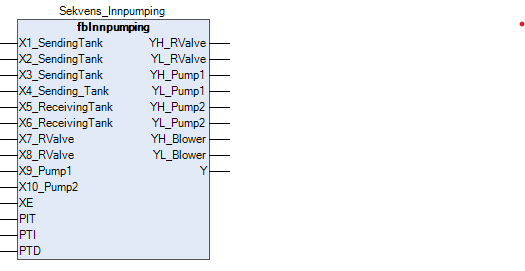
\includegraphics[width=1\textwidth]{Bilder/fbInnpumping.png}
        \caption{Innpumping}\label{fig:fbInnpumping}
    \end{subfigure}
    \hfill
    \begin{subfigure}[b]{0.3\textwidth}
        \centering
        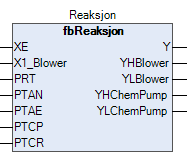
\includegraphics[width=1\textwidth]{Bilder/fbReaksjon.png}
        \caption{Reaksjon}\label{fig:fbReaksjon}
    \end{subfigure}
    \caption{Tilstandslogikk blokker implmentert i programmet}\label{fig:ReaksjonsFasen}
\end{figure}



